The ESMoL modeling tools support the entire process of creating embedded systems software, as described in \cite{pvknks_09}.  An understanding of the steps involved in importing and annotating an ESMoL model to prepare it for TrueTime generation is important.  The complete process for modeling and generation includes the following steps: (1) Import controller design from Simulink (2) Define components and message types (3) Generate component functional code (4) Create deployment hardware configuration (5) Deploy components and messages (6) Calculate time-triggered schedule (7) Synthesize the TrueTime model.

The first step for our example is importing the source controller model from Simulink into the ESMoL modeling environment.  The dataflow semantics of the original Simulink model are preserved and are fully represented within the ESMoL model.  Software components in ESMoL are defined by creating references to Simulink subsystem blocks and to input and output message types.  Instances of these software components correspond to individual run-time tasks.  Each task has logical execution time semantics \cite{hhk_01}, which means that all input messages are available before a task consuming them is released, and output messages of the task are sent at precisely defined points in time, after the task has finished.  Message types and their data elements must also be defined.

Once components and message types are defined, a model interpreter synthesizes platform-independent functional code.  The internal dataflow representation of each component is converted into synchronous C-code blocks which will be executed on top of a thin virtual machine that implements the TTA execution semantics. As will be discussed in Section 3, this functional C-code is complied together with a layer of generated ``glue code'', acting as the TTA virtual machine, and together they are directly incorporated into the TrueTime model.

The next step is to define the deployment platform hardware configuration.  In our example the deployment platform consists of a Gumstix Verdex embedded processing module with a Robostix I/O expansion board, as shown in Fig. \ref{fig:platform}.  They are connected via an $I^{2}C$ bus over which time-triggered communications are sent.
\begin{figure}[ht]
\centering
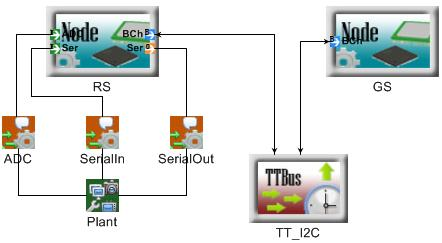
\includegraphics[width=\columnwidth]{figures/platform.jpg}
    \caption{Robostix-Gumstix platform with time-triggered communications bus}
    \label{fig:platform}
\end{figure}

Next, instances of software components are mapped onto the platform.  This step defines the deployment of software onto hardware.  Multiple instances of a particular component may be deployed.  Messages are mapped to I/O ports on the hardware to define channels via which they will be communicated.  The deployment model is used to determine the configuration of TrueTime kernel and network blocks and their relationship and interaction with the plant model.  The deployment of our example quad-rotor components onto our hardware platform is shown in Fig. \ref{fig:deployment}.
\begin{figure}[ht]
\centering
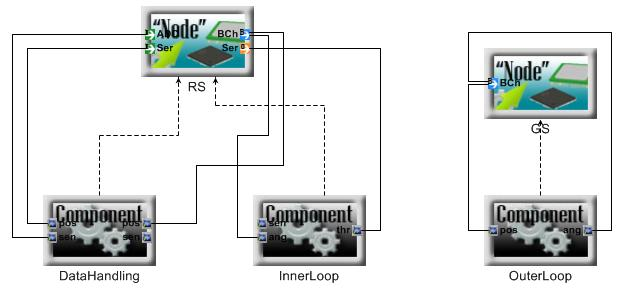
\includegraphics[width=\columnwidth]{figures/deployment.jpg}
    \caption{Deployment of components onto hardware and mapping of ports to communication channels}
    \label{fig:deployment}
\end{figure}

The final step necessary before a TrueTime model can be generated is to execute an off-line schedulability analysis.  Automated schedulability analysis begins with the transformation of the ESMoL model into a scheduler configuration file.  The configuration file contains an abstract version of the design, limited to information about platform connectivity, assignment of tasks to processors, routing of messages through buses, and timing specifications. The ESMoL static scheduler\cite{pks_09} uses this abstract specification to build a finite-domain integer constraint problem, which is solved using the Gecode constraint logic programming library\cite{tools:gecode}.  Details about the scheduler are documented in \cite{pks_09}, though the approach is a refinement of the constraint formulation first described by Schild and W{\"u}rtz\cite{sched:offline}.

The constraint problem models dependencies between tasks and messages, exclusive use of processors and buses, and timing constraints (i.e., maximum acceptable latency between tasks).  If the problem is feasible then a solution will satisfy the specified timing requirements and will contain start times for each of the tasks and messages.  Another automated tool writes the schedule start times to fields in the original model, so that start time information can be used during platform-specific code generation steps.  Infeasible problems are reported as such.

Once a source controller has been imported, components and message types defined, the component functional code generated, a deployment hardware configuration created, components and messages deployed and a time-triggered schedule created, then the ESMoL model is prepared to have the TrueTime model synthesized.